\chapter{等额年金}
\begin{introduction}
	\item 每年支付m次的年金
	\item 连续支付的等额年金
\end{introduction}
\section{符号一览}
\noindent$a_{\angles{n}},s_{\angles{n}}$\\	$\ddot{a}_{\angles{n}}$\\$\ddot{s}_{\angles{n}}$
\section{等额年金}
\begin{definition}{年金的终值与现值}
\noindent $a_{\angles{n}},s_{\angles{n}}$\\
$s_{\angles{n}}=a_{\angles{n}}(1+i)^{n}=\frac{(1+i)^{n}-1}{i}$
\end{definition}
\begin{definition}{Accumulated Value of an $n$ -Payment Annuity-Immediate of 1 Per Period}

	The symbol $s_{\angles{n}}$ denotes the accumulated value, at the time of (and including) the final payment of a series of $n$ payments of 1 each made at equally spaced intervals of time, where the rate of interest per payment period is $i$
	$\begin{aligned}
	s_{\angles{n}} &=(1+i)^{n-1}+(1+i)^{n-2}+\cdots+(1+i)+1 \\
	&=\sum_{t=0}^{n-1}(1+i)^{t}=\frac{(1+i)^{n}-1}{i}
	\end{aligned}$
\end{definition}
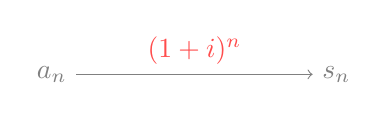
\begin{tikzpicture}
\draw [color=black!50,->](0,0) node[left]{$a_{\angles{n}}$}-- node [color=red!70,pos=0.5,above,sloped]{$(1+i)^n$}(3,0) node[right]{$s_{\angles{n}}$};
    \end{tikzpicture} \\
\noindent $a_{\angles{n}}=v+v^2+v^3+\dots+v^n=\frac{1-v^n}{i}=\frac{1-\frac{1}{(1+i)^n}}{i}=\frac{1-v^n}{\frac{1}{v}-1}$\\
\begin{lstlisting}[language={python}]
#wolframalpha
(1-(1/(1+i)^n))/i=(1-v^n)/(1/v-1)
\end{lstlisting}
$\ddot{a}_{\angles{n}}=\frac{1-v^n}{d}$ \\
$s_{\angles{n}}=a_{\angles{n}}(1+i)^{n}=\frac{(1+i)^{n}-1}{i}$\\
$\ddot{s}_{\angles{n}}=\ddot{a}_{\angles{n}}(1+i)^{n}=\frac{(1+i)^{n}-1}{d}$
\begin{property}
$1=i{a}_{\angles{n}}+v^n$
\end{property}
\begin{property}
$$\begin{array}{l}
\ddot{a}_{\angles{n}}=a_{\angles{n}} \times(1+i) \\
\ddot{a}_{\angles{n} }=a_{\angles{n-1} |+1 \\
\ddot{S}_{\angles{n} }=S_{\bar{n}} \times(1+i) \\
\ddot{S}_{\angles{n}}=S_{\angles{n+1} }-1
\end{array}$$
\end{property}
 \begin{definition}{每年支付m次年金}
\noindent ${a}_{\angles{n}}^{(m)}=\frac{1-v^n}{i^{(m)}}$ 
 \end{definition}
 \section{永续年金(Perpetuity)}
 期初付永续年金的现值
\[
\ddot{a}_{\angles{\infty}}=1+v+v^{2}+\cdots=\frac{1}{1-v}=\frac{1}{1-v}=\frac{1}{d}
\]
期末付永续年金的现值
\[
a_{\angles{\infty}}=v+v^{2}+\cdots=\frac{1}{1-v}=\frac{v}{1-v}=\frac{v}{d}=\frac{v}{i v}=\frac{1}{i}
\]
与有限年金的联系
\[
\begin{array}{c}
\ddot{a}_{\angles{\infty}}=\lim _{n \rightarrow \infty} \ddot{a}_{\pi}=\lim _{n \rightarrow \infty} \frac{1-v^{n}}{d}=\frac{1}{d} \\
a_{\angles{n}}=\frac{1-v^{n}}{i}=\frac{1}{i}-v^{n} \frac{1}{i}=a_{\angles{\infty}}-v^{n} a_{\angles{\infty}} \Leftrightarrow a_{\infty}=a_{\angles{\infty}}+v^{n} a_{\angles{\infty}}
\end{array}
\]
对期初付年金也有相应的关系: $\ddot{a}_{\angles{\infty}}=\ddot{a}_{\pi}+v^{n} \ddot{a}_{\angles{\infty}}$
